\chapter{Conceitos Fundamentais de Sistemas Elétricos de Potência}

Este capítulo apresenta os conceitos fundamentais utilizados no desenvolvimento da plataforma proposta. Inicialmente, são abordadas noções gerais sobre sistemas elétricos de potência, com destaque para as grandezas elétricas utilizadas no projeto. Em seguida, são discutidos os curtos-circuitos em sistemas elétricos, os princípios da proteção, as funções de relés implementadas na plataforma, o padrão COMTRADE e os fundamentos de processamento digital de sinais aplicados a relés digitais.

A fundamentação teórica apresentada neste capítulo tem como objetivo estabelecer a base necessária para compreender a arquitetura do sistema desenvolvido, no qual sinais de tensão e corrente provenientes de simulações são reproduzidos em bancada e utilizados para avaliação de algoritmos de proteção.

\section{Sistemas elétricos de potência}

Um sistema elétrico de potência pode ser entendido como o conjunto de instalações e equipamentos responsáveis pela geração, transmissão, distribuição e utilização da energia elétrica. Em sua estrutura básica, a energia é produzida em unidades geradoras, transportada por linhas de transmissão em níveis elevados de tensão, reduzida em subestações e finalmente entregue aos consumidores por redes de distribuição.

\begin{figure}[H]
  \centering
  \caption{Diagrama unifilar de um sistema elétrico de potência}
  \label{fig:diagrama-sep}
  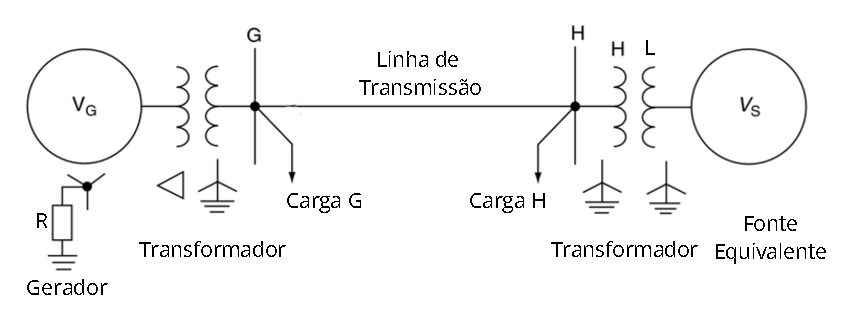
\includegraphics[width=0.94\textwidth]{figuras/sistema_eletrico_potencia_v2_cortado.pdf}
  \legend{Fonte: Adaptado de \citeonline{blackburn2006protective}.}
\end{figure}

A operação desses sistemas exige o equilíbrio contínuo entre geração e carga, além da manutenção de grandezas como tensão, corrente, frequência e potência dentro de limites adequados. Alterações bruscas de carga, falhas em equipamentos, descargas atmosféricas, curtos-circuitos e manobras podem provocar perturbações que afetam a estabilidade, a segurança e a continuidade do fornecimento de energia elétrica \cite{kundur1994power,glover2017power}.

No contexto deste trabalho, as grandezas mais importantes são tensão, corrente, potência, impedância e frequência. Para sinais senoidais em regime permanente, a tensão instantânea pode ser representada por:

\begin{equation}
  v(t) = V_m \sin(\omega t + \theta),
  \label{eq:tensao-instantanea}
\end{equation}

\noindent em que $V_m$ é o valor de pico, $\omega = 2\pi f$ é a frequência angular e $\theta$ é o ângulo de fase. O valor eficaz de uma grandeza senoidal é dado por:

\begin{equation}
  V_{\text{rms}} = \frac{V_m}{\sqrt{2}}.
  \label{eq:vrms}
\end{equation}

Em sistemas trifásicos equilibrados, as potências ativa, reativa e aparente podem ser expressas por:

\begin{align}
  P &= \sqrt{3} V_L I_L \cos\varphi, \label{eq:potencia-ativa}\\
  Q &= \sqrt{3} V_L I_L \sin\varphi, \label{eq:potencia-reativa}\\
  S &= \sqrt{3} V_L I_L, \label{eq:potencia-aparente}
\end{align}

\noindent em que $V_L$ é a tensão de linha, $I_L$ é a corrente de linha e $\varphi$ é o ângulo entre tensão e corrente. A impedância elétrica, por sua vez, pode ser representada por:

\begin{equation}
  Z = R + jX = \frac{\bar{V}}{\bar{I}},
  \label{eq:impedancia}
\end{equation}

\noindent sendo $\bar{V}$ e $\bar{I}$ os fasores de tensão e corrente. Essa relação é particularmente importante para a função de distância, pois a impedância aparente vista pelo relé é calculada a partir dos fasores medidos.

No projeto desenvolvido, os sinais de tensão e corrente são gerados por simulações computacionais, convertidos para COMTRADE e reproduzidos em bancada. Portanto, as equações apresentadas servem de base para a interpretação das amostras reproduzidas e para o cálculo das grandezas utilizadas pelos algoritmos de proteção.

\section{Curtos-circuitos em sistemas elétricos de potência}

O curto-circuito é uma das condições anormais mais relevantes em sistemas elétricos de potência. Ele ocorre quando há uma conexão de baixa impedância entre pontos que deveriam permanecer eletricamente separados. Como consequência, podem surgir correntes elevadas, afundamentos de tensão e esforços térmicos e mecânicos capazes de danificar equipamentos e comprometer a operação do sistema \cite{anderson1999power,blackburn2006protective}.

Os principais tipos de curto-circuito são:

\begin{itemize}
  \item curto-circuito trifásico, envolvendo simultaneamente as três fases;
  \item curto-circuito bifásico, envolvendo duas fases;
  \item curto-circuito bifásico-terra, envolvendo duas fases e a terra;
  \item curto-circuito monofásico-terra, envolvendo uma fase e a terra.
\end{itemize}

As faltas trifásicas são classificadas como simétricas, pois, idealmente, preservam o equilíbrio entre as fases. Já as faltas monofásicas, bifásicas e bifásicas-terra são assimétricas e exigem análise por componentes simétricas. Embora a falta trifásica não seja a mais frequente em sistemas reais, ela é uma das mais severas e é amplamente utilizada em estudos iniciais de curto-circuito e proteção.

\begin{figure}[H]
  \centering
  \caption{Representação simplificada de uma falta trifásica em um sistema elétrico}
  \label{fig:falta-trifasica}
  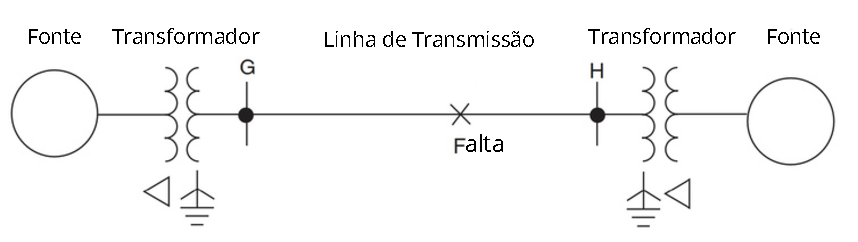
\includegraphics[width=0.92\textwidth]{figuras/SEP_falta_br_cortado.pdf}
  \legend{Fonte: Adaptado de \citeonline{blackburn2006protective}.}
\end{figure}

Para uma falta trifásica, a análise pode ser feita por fase, utilizando o equivalente de Thévenin visto do ponto de falta. A corrente de curto-circuito trifásico é dada por:

\begin{equation}
  I_{cc,3\phi} = \frac{V_{\text{th}}}{Z_{\text{th}} + Z_f},
  \label{eq:icc-trifasico}
\end{equation}

\noindent em que $V_{\text{th}}$ é a tensão de Thévenin por fase, $Z_{\text{th}}$ é a impedância equivalente do sistema até o ponto de falta e $Z_f$ é a impedância da falta. Para uma falta sólida, em que $Z_f \approx 0$, a expressão pode ser aproximada por:

\begin{equation}
  I_{cc,3\phi} \approx \frac{V_{LL}}{\sqrt{3}Z_{\text{th}}},
  \label{eq:icc-solido}
\end{equation}

\noindent sendo $V_{LL}$ a tensão de linha no ponto analisado antes da falta. A potência de curto-circuito trifásica associada pode ser calculada por:

\begin{equation}
  S_{cc,3\phi} = \sqrt{3}V_{LL}I_{cc,3\phi}.
  \label{eq:scc}
\end{equation}

Para faltas assimétricas, as expressões utilizam as impedâncias de sequência positiva, negativa e zero. Por exemplo, para uma falta monofásica-terra, a corrente de falta pode ser expressa por:

\begin{equation}
  I_f = \frac{3V_{\text{fase}}}{Z_1 + Z_2 + Z_0 + 3Z_f}.
  \label{eq:falta-monofasica}
\end{equation}

Neste trabalho, o destaque é dado à falta trifásica, pois ela permite validar a cadeia principal da plataforma com menor complexidade matemática: geração da oscilografia, conversão para COMTRADE, reprodução dos sinais, aquisição pela ESP32 receptora e avaliação das funções de proteção.

\section{Proteção de sistemas elétricos de potência}

A proteção de sistemas elétricos de potência tem como finalidade identificar condições anormais de operação e comandar a isolação seletiva do trecho defeituoso. Para isso, são empregados dispositivos como transformadores de corrente, transformadores de potencial, relés de proteção, disjuntores e sistemas de comunicação e supervisão.

Um sistema de proteção deve atender a critérios fundamentais. A seletividade está relacionada à capacidade de isolar apenas a parte defeituosa do sistema. A sensibilidade indica a capacidade de detectar faltas dentro da zona protegida. A velocidade está associada ao tempo necessário para detectar e eliminar a falta. A confiabilidade envolve a atuação correta quando necessária e a não atuação em situações indevidas \cite{anderson1999power,horowitz2014power}.

Com a evolução dos relés eletromecânicos para relés estáticos e digitais, tornou-se possível implementar múltiplas funções de proteção em um mesmo equipamento. Relés digitais utilizam amostras de sinais de tensão e corrente, realizam processamento numérico e aplicam lógicas configuráveis para determinar se determinada condição exige atuação \cite{phadke2009computer}. Essa característica é explorada neste trabalho por meio da emulação de funções de proteção em uma plataforma embarcada.

\section{Funções de relés de proteção}

As funções de proteção são frequentemente identificadas por números padronizados, conforme a norma IEEE C37.2, que define números e acrônimos para dispositivos e funções utilizados em sistemas elétricos, subestações e instalações de geração \cite{ieee_c37_2_2022}. Essa padronização facilita a documentação técnica, a interpretação de diagramas e a comunicação entre profissionais da área.

No projeto desenvolvido, as funções de relés são tratadas como algoritmos configuráveis. A lógica básica de decisão pode ser representada por uma comparação entre a grandeza medida, extraída das amostras, e um valor de ajuste definido pelo usuário. Em geral, a atuação pode ser expressa por:

\begin{equation}
  \text{atuação} =
  \begin{cases}
    1, & \text{se a condição de atuação permanece verdadeira por } t \geq T_{\text{ajuste}},\\
    0, & \text{caso contrário}.
  \end{cases}
  \label{eq:trip-generico}
\end{equation}

\noindent A seguir, são descritas as principais funções consideradas no contexto da plataforma.

\subsection{Relé de subtensão}

O relé de subtensão, identificado pelo número ANSI 27, atua quando a tensão medida permanece abaixo de um valor previamente ajustado. Essa função é utilizada para detectar afundamentos de tensão, perda de alimentação, falhas em barras, problemas de excitação em máquinas ou condições que possam prejudicar a operação adequada de cargas e equipamentos.

Uma forma usual de parametrização é definir o ajuste em valor por unidade:

\begin{equation}
  V_{pu} = \frac{V_{\text{medido}}}{V_{\text{nominal}}}.
  \label{eq:vpu}
\end{equation}

\noindent Em uma proteção com dois estágios, as condições podem ser representadas por:

\begin{equation}
  V_{pu} \leq V_{27,i}\quad\text{(instantânea)},\qquad
  V_{pu} \leq V_{27,t}\ \text{por}\ t\geq T_{27}\quad\text{(temporizada)}.
  \label{eq:subtensao}
\end{equation}

O estágio temporizado responde a uma subtensão moderada persistente, enquanto o estágio instantâneo é reservado a uma tensão remanescente mais baixa e, portanto, mais crítica. O \textit{pickup} é identificado assim que um ciclo fasorial válido cruza o limiar; a temporização condiciona o \textit{trip}, não a detecção da condição.

\subsection{Relé de sobretensão}

O relé de sobretensão, identificado pelo número ANSI 59, atua quando a tensão medida excede um valor de ajuste. Essa função é aplicada na proteção de equipamentos contra elevações anormais de tensão, que podem ocorrer em rejeição de carga, manobras, falhas de regulação ou sobretensões temporárias.

Utilizando a mesma representação em por unidade da Equação \ref{eq:vpu}, os dois estágios podem ser expressos por:

\begin{equation}
  V_{pu} \geq V_{59,i}\quad\text{(instantânea)},\qquad
  V_{pu} \geq V_{59,t}\ \text{por}\ t\geq T_{59}\quad\text{(temporizada)}.
  \label{eq:sobretensao}
\end{equation}

O estágio temporizado responde a uma elevação moderada e persistente, enquanto o estágio instantâneo atua diante de uma sobretensão mais severa. Em uma plataforma didática, essa separação permite comparar a influência conjunta da magnitude e do tempo sobre a decisão do relé.

\subsection{Relé de sobrecorrente}

O relé de sobrecorrente é uma das funções mais utilizadas em sistemas de proteção. Ele atua quando a corrente medida ultrapassa um valor de \textit{pickup} previamente definido. De acordo com a aplicação, pode assumir forma instantânea, associada ao número ANSI 50, ou temporizada, associada ao número ANSI 51 \cite{blackburn2006protective,ieee_c37_2_2022}.

A condição de atuação instantânea pode ser representada por:

\begin{equation}
  I_{\text{medido}} \geq I_{50,\text{pickup}}.
  \label{eq:sobrecorrente-50}
\end{equation}

Para a função temporizada, define-se normalmente um múltiplo da corrente de \textit{pickup}:

\begin{equation}
  M = \frac{I_{\text{medido}}}{I_{51,\text{pickup}}}.
  \label{eq:multiplo-corrente}
\end{equation}

\noindent Em curvas inversas, o tempo de atuação diminui conforme o múltiplo de corrente aumenta. Uma forma genérica de representar esse comportamento é:

\begin{equation}
  t_{\text{op}} = TMS \left(\frac{A}{M^p - 1} + B \right),
  \label{eq:curva-inversa}
\end{equation}

\noindent em que $TMS$ é o multiplicador de tempo e $A$, $B$ e $p$ são constantes associadas ao tipo de curva adotada. Em uma falta trifásica, a elevação da corrente é um dos efeitos mais evidentes, tornando a função de sobrecorrente especialmente adequada para demonstrações didáticas na plataforma.

\subsection{Relé direcional}

O relé direcional, frequentemente associado à função ANSI 67 quando aplicado à sobrecorrente direcional, utiliza informações de magnitude e fase para determinar o sentido do fluxo de corrente de falta. Essa função é necessária em sistemas nos quais a corrente pode circular em mais de uma direção, como redes malhadas, linhas paralelas, sistemas com geração distribuída ou alimentadores com múltiplas fontes.

Diferentemente de uma proteção de sobrecorrente simples, a proteção direcional não se baseia apenas na intensidade da corrente. Ela também avalia a relação angular entre uma grandeza de operação, normalmente a corrente, e uma grandeza de polarização, normalmente a tensão \cite{horowitz2014power,blackburn2006protective}. Uma forma simplificada de representar o critério direcional é:

\begin{equation}
  \left|\operatorname{ang}(\bar{I}) - \operatorname{ang}(\bar{V}) - \theta_{\text{ref}}\right| \leq \Delta\theta,
  \label{eq:criterio-direcional}
\end{equation}

\noindent em que $\theta_{\text{ref}}$ é o ângulo de referência ou máximo torque e $\Delta\theta$ é a janela angular de atuação. Outra interpretação equivalente utiliza o sinal da potência ativa ou da potência direcional:

\begin{equation}
  P_{\text{dir}} = \operatorname{Re}\{\bar{V}\bar{I}^{*}\}.
  \label{eq:potencia-direcional}
\end{equation}

No contexto deste trabalho, a função direcional reforça a importância da estimação fasorial. Para determinar a direção da falta, não basta conhecer apenas o valor eficaz da corrente; é necessário estimar também os ângulos das grandezas elétricas. Em faltas trifásicas, essa função pode ser combinada com a proteção de distância para permitir ou bloquear a atuação dependendo do sentido estimado da falta.

\subsection{Relé de distância}

O relé de distância, identificado pelo número ANSI 21, é amplamente utilizado na proteção de linhas de transmissão. Seu princípio de funcionamento baseia-se na estimação da impedância aparente vista pelo relé, calculada a partir da relação entre os fasores de tensão e corrente. Quando a impedância estimada entra em uma região de operação previamente definida, o relé interpreta que a falta está dentro de sua zona de proteção \cite{anderson1999power,horowitz2014power}.

A impedância aparente é calculada por:

\begin{equation}
  Z_{\text{app}} = \frac{\bar{V}}{\bar{I}} = R_{\text{app}} + jX_{\text{app}}.
  \label{eq:zapp}
\end{equation}

Em linhas de transmissão, os alcances de zona podem ser definidos como frações da impedância da linha:

\begin{align}
  Z_1 &= k_1 Z_L, \label{eq:zona1}\\
  Z_2 &= k_2 Z_L, \label{eq:zona2}
\end{align}

\noindent em que $Z_L$ é a impedância total da linha e $k_1$ e $k_2$ são fatores de alcance. Em uma característica do tipo mho, por exemplo, a região de atuação pode ser descrita de forma simplificada por:

\begin{equation}
  (R_{\text{app}} - R_c)^2 + (X_{\text{app}} - X_c)^2 \leq r^2,
  \label{eq:mho}
\end{equation}

\noindent em que $(R_c,X_c)$ representa o centro da característica no plano $R$-$X$ e $r$ é o raio da região de operação.

Na plataforma desenvolvida, a função de distância permite estudar a relação entre tensão, corrente e impedância aparente em condições de falta. Para faltas trifásicas, a estimação de $Z_{\text{app}}$ tende a ser mais direta, pois o sistema permanece equilibrado em termos ideais. Além disso, a interação com a função direcional possibilita a análise de lógicas de proteção mais próximas das utilizadas em sistemas reais.

\section{Arquivos COMTRADE}

O padrão COMTRADE é utilizado para armazenar e intercambiar dados transitórios e registros oscilográficos de sistemas elétricos de potência. Sua definição normativa aparece na IEEE C37.111 \cite{ieee_comtrade}. A IEC 60255-24 apresenta a norma equivalente para o mesmo formato \cite{iec_60255_24_2013}. Ele estabelece uma forma comum de representar dados provenientes de registradores digitais de perturbação, relés de proteção, simulações computacionais e sistemas de medição.

De maneira geral, um registro COMTRADE é composto por um arquivo de configuração, com extensão \texttt{.cfg}, e um arquivo de dados, com extensão \texttt{.dat}. O arquivo \texttt{.cfg} descreve informações como identificação do registro, canais analógicos e digitais, unidades, fatores de escala, frequência nominal, taxa de amostragem e formato dos dados. O arquivo \texttt{.dat} contém as amostras propriamente ditas, associadas aos instantes de tempo correspondentes.

Para canais analógicos, a conversão entre o valor armazenado e a grandeza de engenharia pode ser representada por:

\begin{equation}
  x_{\text{eng}} = a x_{\text{raw}} + b,
  \label{eq:escala-comtrade}
\end{equation}

\noindent em que $x_{\text{raw}}$ é o valor registrado no arquivo de dados, $a$ e $b$ são coeficientes definidos no arquivo de configuração e $x_{\text{eng}}$ é a grandeza convertida para sua unidade física. O instante associado à amostra pode ser obtido a partir do índice temporal ou do carimbo de tempo informado no registro.

Neste trabalho, o COMTRADE desempenha papel central, pois permite conectar o ambiente de simulação ao sistema embarcado. As faltas simuladas no Simulink geram sinais de tensão e corrente, que são convertidos para arquivos \texttt{.cfg} e \texttt{.dat}. Em seguida, esses arquivos são validados, decodificados e transformados em amostras apropriadas para envio à ESP32 geradora, que reproduz os sinais por meio do DAC MCP4728.

O uso do COMTRADE também fortalece o caráter acadêmico e aplicado da plataforma, uma vez que esse padrão é empregado na análise de eventos elétricos reais. Assim, os estudantes têm contato com um formato de dados utilizado em estudos de proteção, análise de faltas e avaliação de desempenho de sistemas elétricos. Além disso, a utilização de um padrão reconhecido facilita a futura expansão do projeto para registros de outras fontes, como \textit{softwares} de simulação, registradores digitais ou relés comerciais.

\section{Processamento de sinais em relés digitais}

Relés digitais operam a partir da amostragem de sinais analógicos de tensão e corrente. Após a conversão analógico-digital, as amostras são processadas para estimar grandezas úteis à tomada de decisão, como valor eficaz, fasores, potência, impedância aparente, frequência e componentes simétricas. A qualidade desse processamento influencia diretamente a segurança e a confiabilidade da atuação do relé.

Em condições ideais de regime permanente, os sinais de tensão e corrente de um sistema elétrico podem ser representados por senoides na frequência fundamental, geralmente \SI{50}{\hertz} ou \SI{60}{\hertz}. Entretanto, durante faltas e transitórios, esses sinais podem conter componentes contínuas decrescentes, harmônicas, ruídos e distorções. Por esse motivo, o processamento utilizado em relés digitais deve ser capaz de extrair informações relevantes mesmo em condições não ideais \cite{phadke2009computer}.

O valor eficaz discreto de uma janela de $N$ amostras pode ser estimado por:

\begin{equation}
  X_{\text{rms}} = \sqrt{\frac{1}{N}\sum_{n=0}^{N-1} x^2[n]}.
  \label{eq:rms-discreto}
\end{equation}

Embora o valor eficaz seja útil para representar a intensidade de um sinal, ele não fornece diretamente a informação de fase. Essa limitação é importante porque diversas funções de proteção dependem da relação angular entre tensão e corrente. A proteção direcional utiliza o ângulo entre grandezas para determinar o sentido da falta, enquanto a proteção de distância depende da relação fasorial entre tensão e corrente para calcular a impedância aparente.

Nesse contexto, a Transformada Discreta de Fourier é amplamente empregada em relés digitais para estimar a componente fundamental dos sinais. Para uma janela de $N$ amostras, o coeficiente associado à componente fundamental pode ser representado por:

\begin{equation}
  X_1 = \frac{2}{N}\sum_{n=0}^{N-1} x[n]e^{-j\frac{2\pi n}{N}}.
  \label{eq:dft-fundamental}
\end{equation}

\noindent A partir desse coeficiente, obtêm-se a amplitude de pico e o ângulo da componente fundamental. Para expressar o fasor em valor eficaz, como ocorre no \textit{firmware} receptor, a magnitude deve ser dividida por $\sqrt{2}$:

\begin{align}
  |\bar{X}_1|_{\mathrm{rms}} &= \frac{1}{\sqrt{2}}\sqrt{\operatorname{Re}(X_1)^2 + \operatorname{Im}(X_1)^2}, \label{eq:magnitude-fasor}\\
  \theta_X &= \arctan\left(\frac{\operatorname{Im}(X_1)}{\operatorname{Re}(X_1)}\right). \label{eq:angulo-fasor}
\end{align}

No projeto desenvolvido, esse processamento permite que as amostras recebidas pela ESP32 receptora sejam convertidas em grandezas úteis aos algoritmos de proteção. Assim, a plataforma não apenas reproduz formas de onda, mas também demonstra o processo de aquisição, filtragem, estimação fasorial e decisão lógica característico de relés digitais.

\section{Conclusão}

Este capítulo apresentou os principais conceitos necessários para compreender o desenvolvimento da plataforma didática proposta. Foram discutidos os fundamentos dos sistemas elétricos de potência, a ocorrência de curtos-circuitos, os princípios da proteção elétrica, as funções de relés consideradas no trabalho, o padrão COMTRADE e o processamento de sinais aplicado a relés digitais.

Também foram introduzidas equações fundamentais de potência, curto-circuito, critérios de atuação de relés, conversão de dados COMTRADE e estimação fasorial por Fourier. A partir dessa base teórica, torna-se possível compreender a metodologia adotada no projeto: gerar sinais de falta por simulação, convertê-los para um formato padronizado, reproduzi-los fisicamente por meio de uma ESP32 geradora e avaliá-los em uma ESP32 receptora com algoritmos de proteção. O capítulo seguinte apresenta a metodologia utilizada para integrar esses elementos na arquitetura da plataforma desenvolvida.
